\lstinputlisting[language=bash,basicstyle=\small]{python_codes/fieldstone_18/keywords}

\begin{center}
Code at \url{https://github.com/cedrict/fieldstone/tree/master/python_codes/fieldstone_18}
\end{center}

\par\noindent\rule{\textwidth}{0.4pt}
%%%%%%%%%%%%%%%%%%%%%%%%%%%%%%%%%%%%%%%%%%%%%%%%%%%%%%%%%%%%%%%%%%%%%%%%%%%%%%%%%%%%%%%%%%%%

The details of the numerical setup are presented in Section \ref{mms1}.

Each element has $m_V=9$ vertices so in total $ndof_V\times m_V=18$ velocity dofs and 
$ndof_P*m_P=4$ pressure dofs. The total number of 
velocity dofs is therefore $NfemV=NV \times ndofV$ while the total number of
pressure dofs is $NfemP=NP\times ndofP$. The total number of dofs is then $Nfem=NfemV+NfemP$.

As a consequence, matrix $\K$ has size $NfemV,NfemV$ and matrix $\G$ has size $NfemV,NfemP$.
Vector $f$ is of size $NfemV$ and vector $h$ is of size $NfemP$.  

The pressure nullspace is removed in two different ways:
(i) by setting $p=p_{th}(L_x,L_y)=-1/6$ on the last node, or (ii)
by imposing (Lagrange multiplier) that $\int_\Omega p \; dV=0$.

\begin{center}
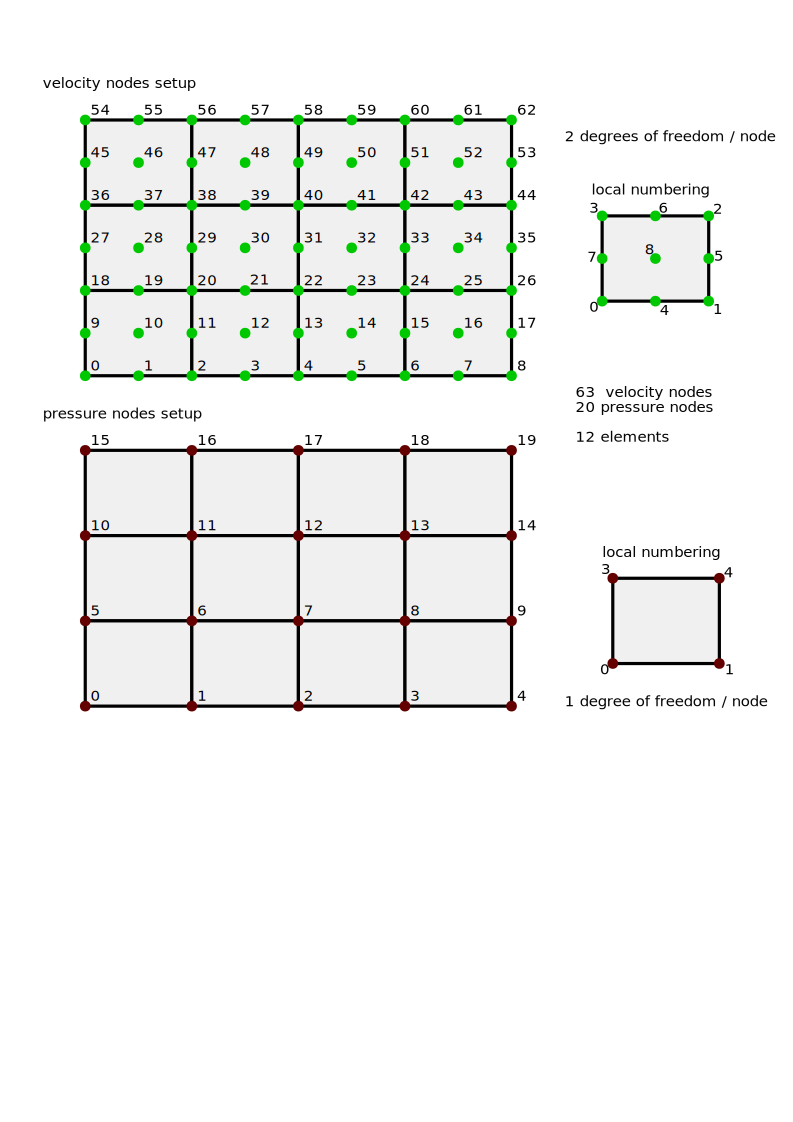
\includegraphics[width=10cm]{python_codes/fieldstone_18/images/q2q1setup}
\end{center}

\begin{center}
\includegraphics[width=7cm]{python_codes/fieldstone_18/results/vel}
\includegraphics[width=7cm]{python_codes/fieldstone_18/results/pressure}\\
{\captionfont velocity and pressure fields for $32\times 32$ elements grid}
\end{center}

\begin{center}
\includegraphics[width=12cm]{python_codes/fieldstone_18/results/errors}\\
{\captionfont Velocity and pressure error convergence for both nullspace removal 
techniques. The zero average pressure approach yields smaller errors.}
\end{center}
